% Fig. 2: overview of RiskIndex.  Compile with XeLaTeX (DejaVu Sans, the font of the plots).
% No legend: the symbols are explained in the caption.
% The drawing is schematic: graph, worlds, RR sets, node ids and bar heights are illustrative.
\documentclass[border=2pt]{standalone}
\usepackage{fontspec}
\setmainfont{DejaVu Sans}
\usepackage{unicode-math}
\setmathfont{DejaVu Math TeX Gyre}
\setmathfont[range={up/{latin,Latin,num}}]{DejaVu Sans}
\setmathfont[range={it/{latin,Latin,greek,Greek}}]{DejaVu Sans Oblique}
\usepackage{tikz}
\usetikzlibrary{arrows.meta,calc,decorations.pathreplacing,positioning}

% palette of the plots (figstyle.py)
\definecolor{pur}{HTML}{7B5FB0}\definecolor{purL}{HTML}{ECE6F6}\definecolor{purM}{HTML}{B9A6DD}
\definecolor{blu}{HTML}{4A86C5}\definecolor{sky}{HTML}{8DB8DD}\definecolor{bluL}{HTML}{E6EFF8}
\definecolor{red}{HTML}{D9705A}\definecolor{sal}{HTML}{EE9A6A}\definecolor{salL}{HTML}{FBE5D8}
\definecolor{ink}{HTML}{2B2B2B}\colorlet{fw}{blu!80}\colorlet{fwL}{blu!45!white}\definecolor{gry}{HTML}{8C8C8C}\definecolor{gryD}{HTML}{555555}
\colorlet{c1}{pur!30}\colorlet{c2}{pur!50}\colorlet{c3}{pur!70}\colorlet{cH}{pur}

\tikzset{
  every node/.style={font=\fontsize{7}{8.2}\selectfont, text=ink, inner sep=1pt},
  ttl/.style={font=\fontsize{6.6}{7.6}\selectfont\bfseries},
  ptitle/.style={font=\fontsize{8.6}{9.8}\selectfont\bfseries},
  hd/.style={font=\fontsize{6.2}{7.2}\selectfont, text=gryD},
  sm/.style={font=\fontsize{6.2}{7.2}\selectfont},
  frame/.style={draw=gry, rounded corners=7pt, line width=0.6pt, dash pattern=on 3.2pt off 2.2pt},
  big/.style={line width=3.4pt, draw=#1, -{Triangle[length=6.5pt,width=9.5pt]}},
  med/.style={line width=2.3pt, draw=#1, -{Triangle[length=4.6pt,width=6.6pt]}},
  onl/.style={font=\fontsize{6.2}{7.2}\selectfont},
  thin/.style={line width=0.5pt, draw=gryD, -{Stealth[length=3pt,width=3pt]}},
  vx/.style={circle, draw=ink, line width=0.35pt, fill=#1, inner sep=0pt, minimum size=4.6pt},
  vxb/.style={circle, draw=ink, line width=0.4pt, fill=#1, inner sep=0pt, minimum size=6.8pt},
  live/.style={line width=0.5pt, draw=ink},
  dead/.style={line width=0.4pt, draw=gry!75, dash pattern=on 1pt off 1.1pt},
  pill/.style={draw=#1, rounded corners=2.2pt, line width=0.5pt, minimum width=0.46cm, minimum height=0.22cm},
  cell/.style={draw=white, line width=0.6pt},
  lg/.style={anchor=west, font=\fontsize{6.4}{7.4}\selectfont},
}

% graph glyph: node coordinates in a 1.62 x 0.95 box
\newcommand{\glyph}[4]{% name x y scale
  \begin{scope}[shift={(#2,#3)}, x=#4cm, y=#4cm]
    \coordinate (#1-1) at (0.00,0.55); \coordinate (#1-2) at (0.40,0.95);
    \coordinate (#1-3) at (0.85,0.70); \coordinate (#1-4) at (0.30,0.12);
    \coordinate (#1-5) at (0.80,0.15); \coordinate (#1-6) at (1.25,0.95);
    \coordinate (#1-7) at (1.25,0.38); \coordinate (#1-8) at (1.62,0.68);
  \end{scope}}
% RR set: x y hit(0/1) {dot colours}
\newcommand{\rr}[4]{%
  \ifnum#3=1 \node[pill=pur, fill=purL] at (#1,#2) {}; \else \node[pill=blu, fill=white] at (#1,#2) {}; \fi
  \foreach \c [count=\j] in {#4} \fill[\c] ({#1-0.22+0.11*\j},#2) circle (0.044);}
% index grid: x0 ytop cell
\newcommand{\igrid}[3]{%
  \foreach \h/\c in {0/c1,1/c2,2/c3,3/cH}
    \foreach \k in {0,...,6}
      \fill[\c!55!white, cell] ({#1+#3*\k},{#2-#3*\h}) rectangle ++(#3,-#3);}
% chain: y colour label {ids}
\newcommand{\chain}[5][white]{%
  \node[sm, text=pur, anchor=east] at (8.98,#2) {$#4$};
  \foreach \id [count=\j] in {#5}
    \node[circle, draw=ink, line width=0.35pt, fill=#3, minimum size=9.8pt, inner sep=0pt,
          font=\fontsize{4.8}{5}\selectfont, text=#1] at (8.84+0.35*\j,#2) {\id};
  \node at (10.53,#2) {$\cdots$};}

\begin{document}
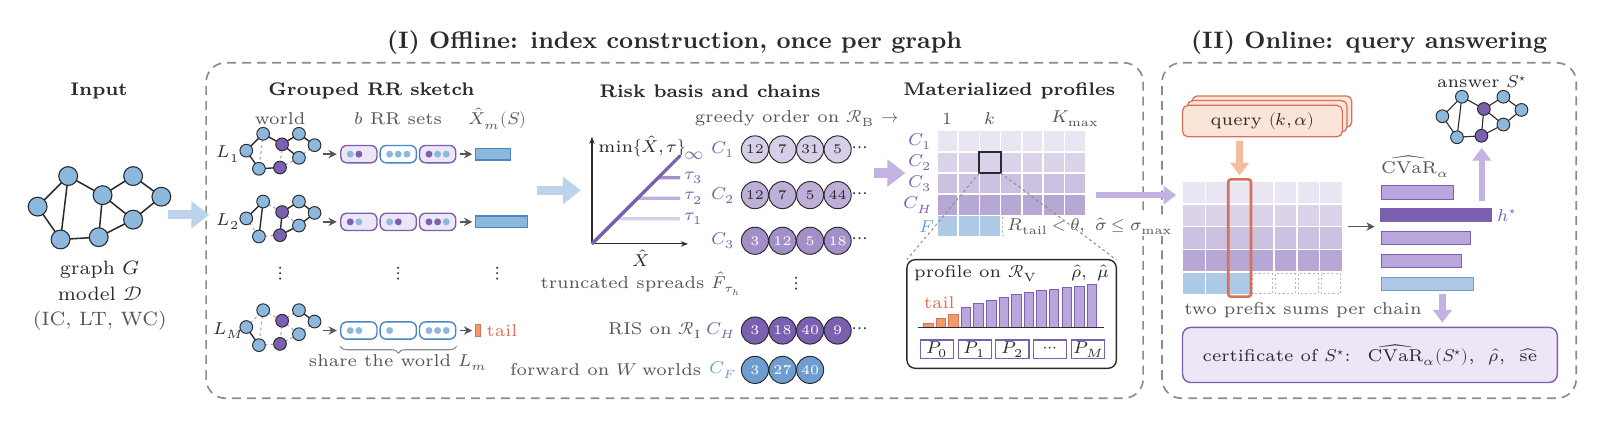
\begin{tikzpicture}[x=1cm,y=1cm]

% =====================================================================  input
\node[ttl] at (0.86,4.62) {Input};
\glyph{in}{0.08}{2.62}{0.97}
\foreach \u/\v in {1/2,2/3,1/4,4/5,2/4,3/5,3/6,3/7,6/8,7/8,5/7}
  \draw[live, line width=0.55pt] (in-\u) -- (in-\v);
\foreach \i in {1,...,8} \node[vxb=sky] at (in-\i) {};
\node[align=center] at (0.87,2.02) {graph $G$\\[1pt]model $\mathcal{D}$\\[1pt]{\color{gryD}(IC, LT, WC)}};

% =====================================================================  frames and titles
\draw[frame] (2.22,0.72) rectangle (14.12,4.98);
\node[ptitle] at (8.17,5.24) {(I) Offline: index construction, once per graph};
\draw[frame] (14.36,0.72) rectangle (19.62,4.98);
\node[ptitle] at (16.99,5.24) {(II) Online: query answering};

% =====================================================================  1. grouped RR sketch
\node[ttl] at (4.32,4.62) {Grouped RR sketch};
\node[hd] at (3.16,4.27) {world};
\node[hd] at (4.66,4.27) {$b$ RR sets};
\node[hd] at (5.92,4.27) {$\hat X_m(S)$};
\foreach \r/\yy/\lab in {1/3.82/{L_1}, 2/2.96/{L_2}, 3/1.58/{L_M}}{
  \glyph{w\r}{2.73}{\yy-0.25}{0.535}
  \node[sm] at (2.50,\yy) {$\lab$};
}
\foreach \u/\v in {1/2,2/3,3/6,6/8,1/4,4/5,3/7} \draw[live] (w1-\u) -- (w1-\v);
\foreach \u/\v in {2/4,3/5,7/8,5/7} \draw[dead] (w1-\u) -- (w1-\v);
\foreach \u/\v in {1/2,2/4,3/5,5/7,7/8,3/6,6/8} \draw[live] (w2-\u) -- (w2-\v);
\foreach \u/\v in {2/3,1/4,4/5,3/7} \draw[dead] (w2-\u) -- (w2-\v);
\foreach \u/\v in {1/4,6/8} \draw[live] (w3-\u) -- (w3-\v);
\foreach \u/\v in {1/2,2/3,4/5,2/4,3/5,3/6,3/7,7/8,5/7} \draw[dead] (w3-\u) -- (w3-\v);
\foreach \r in {1,2,3}{
  \foreach \i in {1,2,4,6,7,8} \node[vx=sky] at (w\r-\i) {};
  \foreach \i in {3,5} \node[vx=pur] at (w\r-\i) {};
}
\node at (3.16,2.30) {$\vdots$};
\foreach \yy in {3.82,2.96,1.58} \draw[thin] (3.70,\yy) -- (3.88,\yy);
\rr{4.16}{3.82}{1}{sky,pur}   \rr{4.66}{3.82}{0}{sky,sky,sky} \rr{5.16}{3.82}{1}{pur,sky,sky}
\rr{4.16}{2.96}{1}{pur,sky}   \rr{4.66}{2.96}{1}{sky,pur}     \rr{5.16}{2.96}{1}{pur,pur,sky}
\rr{4.16}{1.58}{0}{sky,sky}   \rr{4.66}{1.58}{0}{sky}         \rr{5.16}{1.58}{0}{sky,sky,sky}
\node at (4.66,2.30) {$\vdots$};
\draw[decorate, decoration={brace, amplitude=2.5pt, mirror}, line width=0.4pt, gry] (3.92,1.38) -- (5.40,1.38);
\node[hd] at (4.66,1.17) {share the world $L_m$};
\foreach \yy/\len/\c/\cc in {3.82/0.44/sky/blu, 2.96/0.66/sky/blu, 1.58/0.06/sal/red}{
  \draw[thin] (5.44,\yy) -- (5.60,\yy);
  \fill[\c, draw=\cc, line width=0.4pt] (5.64,\yy-0.075) rectangle ++(\len,0.15);
}
\node at (5.92,2.30) {$\vdots$};
\node[sm, text=red, anchor=west] at (5.74,1.58) {tail};

% =====================================================================  2. risk basis and chains
\node[ttl] at (8.62,4.62) {Risk basis and chains};
\begin{scope}[shift={(7.12,2.68)}]
  \draw[line width=0.4pt, ink, -{Stealth[length=2.6pt]}] (0,0) -- (1.22,0);
  \draw[line width=0.4pt, ink, -{Stealth[length=2.6pt]}] (0,0) -- (0,1.36);
  \draw[c1, line width=1.15pt] (0,0) -- (0.32,0.32) -- (1.12,0.32);
  \draw[c2, line width=1.15pt] (0,0) -- (0.58,0.58) -- (1.12,0.58);
  \draw[c3, line width=1.15pt] (0,0) -- (0.84,0.84) -- (1.12,0.84);
  \draw[cH, line width=1.15pt] (0,0) -- (1.12,1.12);
  \node[sm, anchor=north] at (0.62,-0.03) {$\hat X$};
  \node[sm, anchor=north west] at (0.04,1.42) {$\min\{\hat X,\tau\}$};
  \node[sm, text=pur, anchor=west] at (1.13,0.32) {$\tau_1$};
  \node[sm, text=pur, anchor=west] at (1.13,0.58) {$\tau_2$};
  \node[sm, text=pur, anchor=west] at (1.13,0.84) {$\tau_3$};
  \node[sm, text=pur, anchor=west] at (1.13,1.12) {$\infty$};
\end{scope}
\node[hd] at (7.74,2.17) {truncated spreads $\hat F_{\tau_h}$};
\node[hd] at (9.72,4.27) {greedy order on $\mathcal{R}_{\mathrm{B}}$ $\rightarrow$};
\chain[ink]{3.88}{c1}{C_1}{12,7,31,5}
\chain[ink]{3.30}{c2}{C_2}{12,7,5,44}
\chain{2.72}{c3}{C_3}{3,12,5,18}
\node at (9.72,2.18) {$\vdots$};
\chain{1.58}{cH}{C_H}{3,18,40,9}
\node[hd, anchor=east] at (8.55,1.58) {RIS on $\mathcal{R}_{\mathrm{I}}$};
% forward chains (Step 3b): exact spreads on W simulated worlds, small budgets only
\node[sm, text=fw, anchor=east] at (8.98,1.08) {$C_F$};
\foreach \id [count=\j] in {3,27,40}
  \node[circle, draw=ink, line width=0.35pt, fill=fw, minimum size=9.8pt, inner sep=0pt,
        font=\fontsize{4.8}{5}\selectfont, text=white] at (8.84+0.35*\j,1.08) {\id};
\node[hd, anchor=east] at (8.55,1.08) {forward on $W$ worlds};

% =====================================================================  3. materialized profiles
\node[ttl] at (12.42,4.62) {Materialized profiles};
\igrid{11.50}{4.12}{0.27}
\node[hd] at (11.635,4.27) {$1$};
\node[hd] at (12.175,4.27) {$k$};
\node[hd] at (13.255,4.27) {$K_{\max}$};
\foreach \h/\lab in {0/{C_1},1/{C_2},2/{C_3},3/{C_H}} \node[sm, text=pur, anchor=east] at (11.48,4.12-0.27*\h-0.135) {$\lab$};
\foreach \k in {0,1,2} \fill[fwL, cell] ({11.50+0.27*\k},3.04) rectangle ++(0.27,-0.27);
\foreach \k in {3,...,6} \draw[gry!60, line width=0.3pt, dash pattern=on 0.8pt off 0.8pt] ({11.50+0.27*\k+0.02},3.02) rectangle ++(0.23,-0.23);
\node[sm, text=fw, anchor=east] at (11.48,2.905) {$F$};
\node[hd, anchor=west, fill=white, inner sep=0.6pt] at (12.37,2.905) {$R_{\mathrm{tail}}<\theta,\ \hat\sigma\le\sigma_{\max}$};
\draw[ink, line width=0.7pt] (12.04,3.85) rectangle ++(0.27,-0.27);
\draw[gry, line width=0.35pt, dash pattern=on 1pt off 1pt] (12.04,3.58) -- (11.12,2.48);
\draw[gry, line width=0.35pt, dash pattern=on 1pt off 1pt] (12.31,3.58) -- (13.78,2.48);
\draw[ink, line width=0.5pt, rounded corners=3pt, fill=white] (11.12,1.10) rectangle (13.78,2.48);
\node[sm, anchor=north west] at (11.17,2.45) {profile on $\mathcal{R}_{\mathrm{V}}$};
\node[sm, anchor=north east] at (13.73,2.45) {$\hat\rho,\ \hat\mu$};
\foreach \j/\hh in {0/0.10,1/0.21,2/0.30,3/0.45,4/0.55,5/0.62,6/0.69,7/0.74,8/0.79,9/0.83,10/0.87,11/0.91,12/0.94,13/0.98}{
  \pgfmathsetmacro{\xx}{11.33+0.16*\j}
  \ifnum\j<3 \fill[sal, draw=red, line width=0.3pt] (\xx,1.62) rectangle ++(0.12,\hh*0.56);
  \else \fill[purM, draw=pur, line width=0.3pt] (\xx,1.62) rectangle ++(0.12,\hh*0.56); \fi
}
\draw[ink, line width=0.35pt] (11.26,1.62) -- (13.62,1.62);
\node[sm, text=red, anchor=south] at (11.53,1.82) {tail};
\foreach \t [count=\j from 0] in {P_0,P_1,P_2,\cdots,P_M}
  \node[draw=pur, fill=white, line width=0.4pt, minimum width=0.42cm, minimum height=0.24cm, inner sep=0pt, sm]
    at (11.50+0.48*\j,1.34) {$\t$};

% =====================================================================  4. online query
% query workload (top left)
\foreach \d in {2,1}
  \draw[draw=red, fill=salL, rounded corners=2pt, line width=0.45pt] (14.62+0.06*\d,4.04+0.06*\d) rectangle ++(2.03,0.40);
\draw[draw=red, fill=salL, rounded corners=2pt, line width=0.45pt] (14.62,4.04) rectangle ++(2.03,0.40);
\node[onl] at (15.635,4.24) {query $(k,\alpha)$};
% the stored index, column k read by the query (middle left)
\igrid{14.62}{3.48}{0.29}
\foreach \k in {0,1,2} \fill[fwL, cell] ({14.62+0.29*\k},2.32) rectangle ++(0.29,-0.29);
\foreach \k in {3,...,6} \draw[gry!60, line width=0.3pt, dash pattern=on 0.8pt off 0.8pt] ({14.62+0.29*\k+0.02},2.30) rectangle ++(0.25,-0.25);
\draw[red, line width=0.95pt, rounded corners=1pt] (15.20,3.50) rectangle ++(0.29,-1.49);
\node[hd, anchor=west] at (14.60,1.84) {two prefix sums per chain};
% tail estimate of each chain; best chain h* (middle right)
\node[hd, anchor=west] at (17.10,3.66) {$\widehat{\mathrm{CVaR}}_\alpha$};
\foreach \h/\len in {0/0.92,1/1.40,2/1.14,3/1.02}{
  \pgfmathsetmacro{\yy}{3.48-0.29*\h-0.145}
  \ifnum\h=1 \fill[pur, draw=pur] (17.14,\yy-0.085) rectangle ++(\len,0.17);
  \else \fill[purM, draw=pur, line width=0.3pt] (17.14,\yy-0.085) rectangle ++(\len,0.17); \fi
}
\fill[fwL, draw=fw, line width=0.3pt] (17.14,2.175-0.085) rectangle ++(1.18,0.17);
\node[sm, text=pur, anchor=west] at (18.58,3.045) {$h^\star$};
% answer seed set (top right)
\glyph{out}{17.92}{3.96}{0.62}
\foreach \u/\v in {1/2,2/3,1/4,4/5,2/4,3/5,3/6,3/7,6/8,7/8,5/7} \draw[live, line width=0.4pt] (out-\u) -- (out-\v);
\foreach \i in {1,2,4,6,7,8} \node[vx=sky] at (out-\i) {};
\foreach \i in {3,5} \node[vx=pur] at (out-\i) {};
\node[onl] at (18.42,4.74) {answer $S^\star$};
% certificate (bottom, full width)
\draw[draw=pur, fill=purL, rounded corners=3pt, line width=0.5pt] (14.62,0.92) rectangle (19.38,1.62);
\node[onl] at (17.00,1.27) {certificate of $S^\star$:\quad $\widehat{\mathrm{CVaR}}_\alpha(S^\star)$,\ \ $\hat\rho$,\ \ $\widehat{\mathrm{se}}$};

% =====================================================================  flow arrows (straight, one size)
\draw[big=sky!60] (1.74,3.05) -- (2.26,3.05);
\draw[big=sky!60] (6.42,3.36) -- (6.98,3.36);
\draw[big=purM!85] (10.70,3.58) -- (11.10,3.58);
\draw[med=purM!85] (13.52,3.30) -- (14.54,3.30);
\draw[med=sal!65] (15.345,3.99) -- (15.345,3.55);
\draw[thin] (16.72,2.90) -- (17.06,2.90);
\draw[med=purM!85] (18.42,3.22) -- (18.42,3.90);
\draw[med=purM!85] (17.92,2.04) -- (17.92,1.68);

\end{tikzpicture}
\end{document}
